%
% Draft  document primitive.tex
% What are the defining characteristic(s) of a primitive sheep
% relative to a modern Merino sheep
%
 
\documentclass[titlepage]{article}  % Latex2e
\usepackage{graphicx,lscape,subfigure}
\usepackage{bm,longtable}
\usepackage{textcomp}
 

\title{What are the defining characteristics of a primitive sheep relative to a modern Merino sheep}
\author{Neville Jackson}
\date{14 Aug 2017} 

 
\begin{document} 
 
\maketitle      
\tableofcontents

\clearpage
\section{Introduction} 
The question has arisen, in reviewing the document Jackson, Maddocks, Lax, Moore, and Watts (1990)~\cite{jack:90}, of which characteristics would be most appropriate in identifying sheep which are showing signs of reversion to a primitive two-coated fleece type.

It is obvious that we should make some use of the diameters of primary and secondary fibres, but the exact form in which these data should be used, and whether other characteristics (such as primary and secondary follicle densities, shedding follicles, birthcoat coarsness, follicle arrangement, and visibly protruding coarse fibres in the fleece) should also be used, are open to debate. To some extent the practical answer is limited by available data.

\section{Terminology}
We need to be consistent in using the following terms
\begin{description}
\item[kemp] coarse heavily medullated fibres that shed anually or more often
\item[hair] coarse persistantly growing wool fibres. May be medulated but not as heavily medullated as kemp fibres. May shed but not synchronously.
\item[wool] medium to fine fibres. No medullation. Shed in undercoat of wild sheep, but not in modern fine and medium breeds.
\end{description}


\section{Definition of a primitive fleece type}
We refer to the extensive studies of Ryder(1981)~\cite{ryde:81} and Ryder(1992)~\cite{ryde:92}. In summary,
\begin{itemize}
\item wild sheep are two-coated, with coarse long kemp fibres and short fine underwool. 
\item the first domestic sheep ( in the Neolithic (Stone Age) period (10000-3000BC) were similar to wild sheep. Some of the kempy sheep of Africa and India today are survivors of this type.
\item in the Bronze Age (3000-1000 BC) the kemp fibres became finer , while the fine undercoat fibres became slightly coarser. Shedding of the fleece was still necessary ( there were no shears in the Bronze Age), fibres were combed fro the sheep. Modern representative is Hairy Soay
\item  In the Iron Age (1000BC - 700AD  the long kemp fibres became continuous growing long fibres termed "hair", and the fine-medium undercoat also became continuous growing. In some breeds the hairs also became finer. Modern representative is Wooly Soay.
\item modern breeds ( British Longwools, British Shortwools, and fine Merino) are all derived from Iron Age sheep, in the Middle Ages (700AD - 1700AD) by various modifications of the fineness and length of fibres.  All  these modern breeds are continuous growing
\item in tropical Africa and India some survivors of the Bronze Age hairy sheep have actually further reduced the underwool, presumable as an adaptation to tropical conditions.
\item in the New World ( Australia and USA) present day derivatives of the modern European Breeds were developed, mainly by cross breeding followed by selection.
\end{itemize}
The extent of the changes  noted above are shown in a diagram from Ryder(1992)~\cite{ryde:92} in Figure~\ref{fig:ryder}
%\documentclass{article}
%\usepackage{graphicx,subfigure}
%\begin{document}

\begin{figure}[!h]
  \centering
   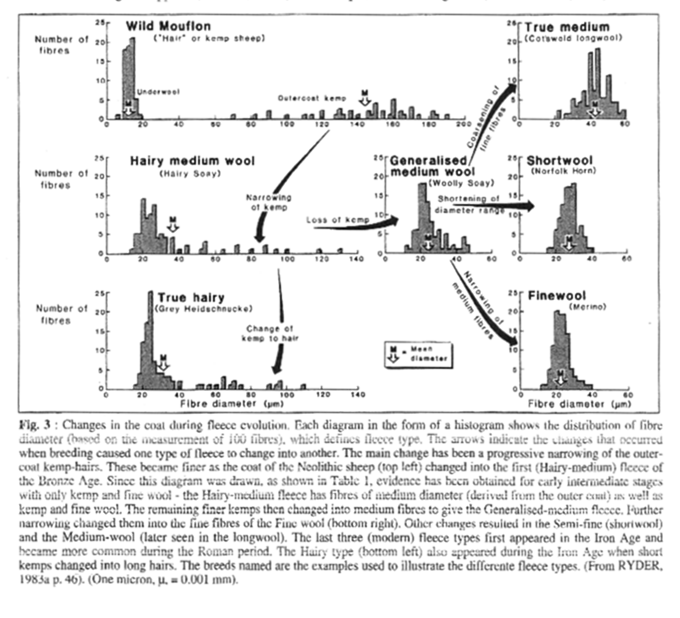
\includegraphics[width=1.0\textwidth]{ryder1crop.png}
%  \includegraphics{fig1.png}
  \caption{Figure copied from Ryder(1992)~\cite{ryde:92}}
  \label{fig:ryder}
\end{figure}

%\end{document}



So Ryder considers that Fine Merino sheep are descended from his "Generalised Medium Wool", which in turn is descended from "Hairy Medium Wool", which in turn is descended from wild sheep. In other words Merinos are descended from primitive domestic sheep of the Bronze and Iron Ages, not from other medieval breeds such as the British Longwools and Shortwools.

This is basically in agreement with the description of Merino evolution given in Fraser and Short(1960)~\cite{fras:60} which was referred to in Jackson et al(1990)~\cite{jack:90} and used as a basis for the statement
\begin{quote}
"The Merino breed is considered to have evolved directly from either wild sheep aor primitive two-coated domestic sheep"
\end{quote}

We present the diagram given by Fraser and Short(1960)~\cite{fras:60} in Figure~\ref{fig:fraser}.
%\documentclass{article}
%\usepackage{graphicx,subfigure}
%\begin{document}

\begin{figure}[!h]
  \centering
   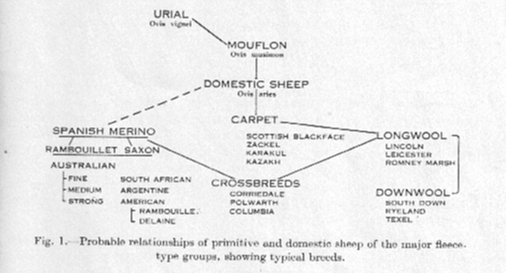
\includegraphics[width=1.0\textwidth]{fraser1crop.png}
%  \includegraphics{fig1.png}
  \caption{Figure copied from Fraser and Short(1960)~\cite{fras:60}}
  \label{fig:fraser}
\end{figure}

%\end{document}



It is basically the same as Ryder, but less supported by data. It comes in turn from an even earlier publication (Von Bergen and Mauersberger(1948)~\cite{vonb:48}. Ryder wants to insert his Generalised Medium Wool in between primitive two coated sheep and the Merino.

What is important here is that the term "primitive domestic sheep" could mean either Stone Age sheep, which are basically unchanged wild sheep, or Bronze Age sheep, which are still two-coated but the outer coat is less medullated and not as coarse. Both the Stone Age and Bronze Age sheep are shedding sheep.   The outer and under coats both shed, but at different times - the undercoat sheds seasonally and all at once, the outer coat fibres shed individually at random times. 

So the term "primitive domestic sheep" is ambiguous.  It is best considered a broad term encompassing all domestic two-coated sheep from the ancient world.

\section{The time scale of Merino evolution}
From Ryder's diagram (Figure~\ref{fig:ryder}) we can put an approximate time scale on the stages of Merino evolution.  This is attempted in Table~\ref{tab:timescale}
%\documentclass{article}
%\usepackage{lscape}
%\begin{document}

\begin{table}[h]
\centering
\caption{Establishing a time scale for the stages of Merino evolution}
\label{tab:timescale}
\vspace{0.1in}
\begin{tabular}{l|l|l|l}  \hline
  Stage &  Chronology &  Years  & Generations \\ \hline
  Wild   & Neolithic (10000-3000BC) & 8000     & 2000 \\
  Hairy Medium Wool & Bronze Age (3000 - 1000BC) & 4000 & 1000 \\
  Generalised Medium Wool & Iron Age (1000BC - 700 AD) & 2100 & 520 \\ \hline
\end{tabular}
\end{table}

%\end{document}

So Ryder is saying that a modern Fine Merino  with a 22.5 micron mean diameter, is about 500 sheep generations removed from a Generalised Medium Wool with a 24.4 micron mean diameter. 

So how long does it take to change mean diameter of a flock by 2 microns? Well with a heritability of 0.4 and a phenotypic standard deviation of 1.4 microns, if one selected for diameter and nothing else one might achieve a selection differential of about 1.3 standard deviations, so the expected response is 
\begin{eqnarray*}
R & = & i h^{2} \sigma \\
  & = & (1.3) (0.4) (1.4) \\
  & = &  0.7
\end{eqnarray*}
 in one generation, which is about 4 years in sheep. So there is certainly plenty of time in 500 years for this amount of change to have occurred. 

However, that is not the whole story. Apart from the change in mean, there are considerable changes in the shape of the distribution between a Generalised Medium Wool and  Merino. Also we do not know from Ryder's data, how the diameters of primary and secondary fibres have changed. We look at this from some more extensive data later on. What is clear, from Ryder, is that mean diameter is not the most important part of the story: the fibre population has components which have changed independently during the breeding of wool sheep.

We also need to look at longer term evolution. Lets say we started with wild sheep, and looked just at the outer coat, witha mean diameter of about 140 microns. To change this to the 20 micron mean of all fibres of a Fine Merino would take, on the above calculation $120/0.7 = 170$ sheep generations - easily achieved in the 2000 sheep generations available between Wild sheep and Merinos. However, this also shows that we could reverse the Merino to Wild sheep in a mere 170 generations. 

Clearly sheep breeders have taken their time over the years, to the extent of taking 10 times longer to achieve a modern fleece quality than would have been required had they concentrated on nothing else. Clearly our assumed selection differential of 1.3 standard deviations ( which comes from a flock with rams replaced annually) is not correct. Ancient flocks probably turned the rams over much more slowly, so the selection differential would have been smaller and the generation interval longer.


There are also changes in characteristics other than fibre diameter. The seasonally shedding undercoat  of Wild sheep and Hairy Medium Wool sheep changed suddenly during the Iron Age to continuous growing fibres. So the secondary follicles all moved into the Anagen phase of the hair growth cycle, and at the same time became slightly coarser. This did not happen to primary follicles. Primary follicles shed asynchronously and aseasonally in all breeds from Wild sheep to Modern Fine Merinos. The only modification to primary fibres has been change from kemp to hair which involves reduction in medullation and reduction in diameter.   The continuous growing fibre modification is clearly not systemic. It appears to have happened relatively rapidly somewhere within the 2000 year span of the Iron Age. 

The first historical records we have of the Merino breed are around the 12th century AD in Medieval Spain (Massy(2007)~\cite{mass:07}. Spanish Merinos were already continuous growing finewool sheep, so we can subtract 1200 years or 300 generations from the timelines in Table~\ref{tab:timescale}.  The Merino breed also differs from all others in having a higher density of secondary follicles, or a higher S/P ratio, and in having the additional secondary follicles formed by branching from other follicles forming a compound follicle, sometimes with as many as 25 branches. The fibres grown by highly branched follicles appear to differ in internal stucture, being less curved, finer, and longer growing.  

\section{The Carter(1968) data on diameter of primary and secondary fibres}
To do anything more objective, we need measurements. Fortunately, there is a comprehensive set of sheep breed skin data, including Dp and Ds, collected by Dr H. B. Carter ( Carter(1968)~\cite{cart:68}). We list the breed means here in Table~\ref{tab:carter68}
%\documentclass{article}
%\usepackage{lscape,longtable}
%\begin{document}

% latex table generated in R 3.2.4 by xtable 1.8-2 package
% Wed Aug 23 20:43:32 2017

\begin{center}
\begin{landscape}
\begin{longtable}{|p{0.4in}|p{0.9in}|p{0.7in}|p{0.5in}|p{0.5in}|p{0.5in}|p{0.5in}|p{0.5in}|p{0.5in}|p{0.5in}|p{0.5in}|p{0.5in}|}
\caption{Listing of breed means from the Carter(1968)~\cite{cart:68} data set} \\
\hline
\label{tab:carter68}
  Flock & Breed & Country & NoSamp & Age & Npsua & Npua & NsovNp & Dp & Ds & Dps & DpovDs \\ 
  \hline
\endfirsthead
\multicolumn{12}{c}%
{\tablename\ \thetable\ -- \textit{Continued from previous page}} \\
\hline
  Flock & Breed & Country & NoSamp & Age & Npsua & Npua & NsovNp & Dp & Ds & Dps & DpovDs \\
\hline
\endhead
\hline
\multicolumn{5}{r}{\textit{Continued on next page}} \\
\endfoot
\hline
\endlastfoot

  1 &  Early Fine Merino &  NSW & 21 &  11-18 & 60.2 & 4.0 & 14.0 & 19.2 & 17.2 & 17.3 & 1.1 \\ 
  2 &  Tas. Fine Merino &  Tas & 21 &  12-14 & 73.3 & 3.5 & 19.6 & 18.3 & 17.8 & 17.9 & 1.0 \\ 
  3 &  Tas. Fine Merino &  Scot & 11 &  12-14 & 62.0 & 3.0 & 20.3 & 21.3 & 20.9 & 20.9 & 1.0 \\ 
  4 &  Tas. Fine Merino &  Tas & 21 &  12-14 & 72.8 & 3.4 & 20.7 & 19.2 & 16.8 & 16.9 & 1.2 \\ 
  5 &  Tas. Fine Merino &  NSW & 20 &  8-9 & 59.9 & 2.5 & 22.8 & 18.4 & 19.8 & 19.7 & 0.9 \\ 
  6 &  Tas. Fine Merino &  Vic & 21 &  14-15 & 79.6 & 3.6 & 21.1 & 19.3 & 16.7 & 16.8 & 1.1 \\ 
  7 &  Tas. Fine Merino &  NSW & 24 &  36 & 48.6 & 2.4 & 19.4 & 19.0 & 18.8 & 18.8 & 1.0 \\ 
  8 &  Tas. Fine Merino &  NSW & 16 &  36 & 46.6 & 2.7 & 16.7 & 20.6 & 18.1 & 18.3 & 1.1 \\ 
  9 &  Tas. Fine Merino &  Scot & 11 &  36 & 54.5 & 2.6 & 20.4 & 21.8 & 21.7 & 21.7 & 1.0 \\ 
 10 &  Vic. Fine Merino &  Vic & 21 &  14-15 & 57.2 & 3.5 & 15.3 & 20.2 & 18.0 & 18.1 & 1.1 \\ 
 11 &  Vic. Fine Merino &  Vic & 11 &  14-15 & 62.3 & 3.7 & 16.0 & 18.3 & 15.9 & 16.1 & 1.2 \\ 
 12 &  Vic. Fine Merino &  Vic & 13 &  14-15 & 76.4 & 3.8 & 19.6 & 15.8 & 15.7 & 15.7 & 1.0 \\ 
 13 &  Vic. Fine Merino &  Vic & 21 &  14-15 & 71.3 & 3.5 & 19.8 & 22.7 & 19.9 & 20.0 & 1.1 \\ 
 14 &  NSW Fine Merino &  NSW & 21 &  10-12 & 87.4 & 3.4 & 24.7 & 19.0 & 17.1 & 17.2 & 1.1 \\ 
 15 &  Non-Peppin Fine-Medium Merino &  NSW & 25 &  60-72 & 43.1 & 2.2 & 20.7 & 23.0 & 22.6 & 22.6 & 1.0 \\ 
 16 &  Non-Peppin Fine-Medium Merino &  NSW & 22 &  60-72 & 50.1 & 2.3 & 21.3 & 22.3 & 21.0 & 21.1 & 1.1 \\ 
 17 &  Non-Peppin Medium Merino &  NSW & 22 &  14-15 & 55.6 & 2.4 & 22.6 & 26.6 & 22.3 & 22.5 & 1.2 \\ 
 18 &  Peppin Medium Merino &  NSW & 30 &  15-18 & 57.1 & 2.8 & 19.7 & 29.8 & 23.7 & 24.0 & 1.3 \\ 
 19 &  Peppin Medium Merino &  NSW & 20 &  15-18 & 63.4 & 3.1 & 19.7 & 25.1 & 17.8 & 18.1 & 1.4 \\ 
 20 &  Peppin Medium Merino &  NSW & 20 &  18-20 & 63.4 & 2.8 & 27.4 & 28.0 & 22.8 & 22.9 & 1.2 \\ 
 21 &  Peppin Medium Merino &  NSW & 20 &  18-20 & 58.6 & 2.4 & 24.2 & 25.6 & 23.2 & 23.3 & 1.1 \\ 
 22 &  Peppin Medium Merino &  Vic & 21 &  14-15 & 72.9 & 3.5 & 20.0 & 21.6 & 17.1 & 17.3 & 1.3 \\ 
 23 &  Peppin Medium Merino &  Vic & 15 &  12-14 & 65.7 & 2.8 & 22.4 & 25.5 & 19.9 & 20.2 & 1.3 \\ 
 24 &  Peppin Medium Merino &  Vic & 11 &  14-15 & 65.2 & 3.4 & 18.5 & 21.1 & 16.8 & 17.0 & 1.3 \\ 
 25 &  Peppin Medium Merino &  Tas & 21 &  12-14 & 79.8 & 4.0 & 19.0 & 22.5 & 19.2 & 19.4 & 1.2 \\ 
 26 &  SA Strong Merino &  SA & 21 &  12-15 & 64.8 & 4.0 & 15.9 & 29.7 & 22.5 & 22.9 & 1.3 \\ 
 27 &  SA Strong Merino &  SA & 21 &  12-15 & 53.5 & 3.0 & 16.8 & 30.8 & 23.7 & 24.1 & 1.3 \\ 
 28 &  SA Strong Merino &  SA & 21 &  12-15 & 53.1 & 2.8 & 18.5 & 32.6 & 24.7 & 25.1 & 1.3 \\ 
 29 &  Early Fine Merino (Rambouillet) &  France & 20 &  12 & 50.4 & 4.1 & 11.5 & 24.3 & 21.1 & 21.3 & 1.1 \\ 
 30 &  Early Fine Merino (Rambouillet) &  France & 18 &  14 & 44.5 & 2.8 & 15.4 & 21.5 & 19.1 & 19.2 & 1.1 \\ 
 31 &  American Rambouillet &  USA & 12 &  18 & 35.2 & 2.4 & 13.9 & 27.2 & 23.4 & 23.7 & 1.2 \\ 
 32 &  American Rambouillet &  Turkey & 21 &  36 & 40.8 & 2.4 & 16.5 & 21.6 & 21.7 & 21.6 & 1.0 \\ 
 33 &  American Merino &  USA & 12 &  18 & 43.0 & 2.5 & 16.0 & 23.3 & 18.9 & 19.2 & 1.2 \\ 
 34 &  American Merino &  Italy &  8 &  24-84 & 40.3 & 3.1 & 12.5 & 19.3 & 17.6 & 17.7 & 1.1 \\ 
 35 &  Debouillet &  USA & 12 &  12 & 44.9 & 3.0 & 14.3 & 21.5 & 16.2 & 16.6 & 1.3 \\ 
 36 &  Merino Tor Mancina &  Italy &  8 &  48-84 & 35.7 & 2.6 & 13.0 & 21.4 & 19.4 & 19.5 & 1.1 \\ 
 37 &  Improved Apulian &  Italy &  8 &  24-84 & 29.3 & 2.3 & 11.8 & 20.7 & 20.4 & 20.4 & 1.0 \\ 
 38 &  German Merinofleischaf &  Turkey & 21 &  36 & 30.5 & 2.1 & 14.0 & 20.6 & 21.3 & 21.1 & 0.9 \\ 
 39 &  German Merinolandschaf &  Turkey & 19 &  36 & 31.5 & 2.7 & 10.7 & 28.5 & 24.3 & 26.4 & 1.1 \\ 
 40 &  Turkish Merino &  Turkey & 21 &  36 & 27.1 & 2.4 & 10.7 & 23.0 & 21.6 & 22.3 & 1.1 \\ 
 41 &  Portuguese Merino &  Portugal & 12 &  24-84 & 23.2 & 3.1 & 6.7 & 26.1 & 23.5 & 23.9 & 1.1 \\ 
 42 &  Polwarth &  NSW & 21 &  14-15 & 52.5 & 3.8 & 12.8 & 23.8 & 19.2 & 19.5 & 1.2 \\ 
 43 &  Polwarth &  NSW & 21 &  14-15 & 54.0 & 4.3 & 11.8 & 23.6 & 21.3 & 21.5 & 1.1 \\ 
 44 &  Polwarth &  Vic & 21 &  13-14 & 44.1 & 2.8 & 15.0 & 26.7 & 23.7 & 23.9 & 1.1 \\ 
 45 &  Polwarth &  Vic & 11 &  14-15 & 46.9 & 3.2 & 13.5 & 21.6 & 17.4 & 17.7 & 1.2 \\ 
 46 &  Targhee &  USA & 12 &  18 & 27.6 & 2.0 & 13.0 & 28.6 & 25.4 & 25.6 & 1.1 \\ 
 47 &  Corriedale &  NSW & 21 &  11-12 & 23.1 & 2.1 & 10.1 & 32.8 & 33.8 & 33.6 & 1.0 \\ 
 48 &  Corriedale &  NSW & 21 &  11-12 & 30.0 & 2.5 & 11.0 & 33.8 & 31.7 & 31.9 & 1.1 \\ 
 49 &  Corriedale &  NSW & 21 &  7-8 & 31.1 & 2.7 & 10.8 & 31.4 & 31.5 & 31.5 & 1.0 \\ 
 50 &  Corriedale &  NSW & 19 &  36 & 19.0 & 1.8 & 9.4 & 37.0 & 30.4 & 31.0 & 1.2 \\ 
 51 &  Corriedale &  Tas & 19 &  36 & 22.3 & 2.0 & 10.5 & 32.7 & 33.8 & 33.7 & 1.0 \\ 
 52 &  Corriedale &  USA & 12 &  12-72 & 15.9 & 1.7 & 8.4 & 29.1 & 26.3 & 26.7 & 1.1 \\ 
 53 &  Columbia &  USA & 12 &  18 & 20.9 & 1.8 & 10.6 & 29.7 & 28.4 & 28.8 & 1.0 \\ 
 54 &  Sopravissano Rossi &  Italy &  8 &  24-84 & 23.4 & 2.4 & 8.6 & 25.6 & 22.7 & 23.0 & 1.1 \\ 
 55 &  Ile-de-France &  France & 14 &  24-96 & 20.3 & 2.5 & 7.1 & 33.2 & 29.3 & 29.7 & 1.1 \\ 
 56 &  Ile-de-France &  Italy &  8 &  24-84 & 12.6 & 1.7 & 6.4 & 27.2 & 27.4 & 27.4 & 1.0 \\ 
 57 &  Southdown &  UK & 18 &  3 & 31.1 & 4.8 & 5.5 & 27.4 & 27.5 & 27.5 & 1.0 \\ 
 58 &  Southdown &  NSW & 21 &  11-12 & 27.8 & 3.9 & 6.3 & 26.1 & 25.2 & 25.4 & 1.0 \\ 
 59 &  Southdown &  UK & 12 &  18 & 16.9 & 2.7 & 5.7 & 34.1 & 32.9 & 33.1 & 1.0 \\ 
 60 &  Dorset Horn &  NSW & 19 &  11-12 & 18.5 & 2.9 & 5.4 & 33.6 & 34.6 & 34.4 & 1.0 \\ 
 61 &  Suffolk &  Vic & 21 &  11-12 & 20.4 & 3.5 & 4.8 & 26.0 & 23.1 & 23.6 & 1.1 \\ 
 62 &  Ryeland &  NSW & 21 &  11-12 & 15.8 & 2.5 & 5.5 & 31.6 & 31.5 & 31.5 & 1.0 \\ 
 63 &  Ryeland &  NSW & 16 &  24 & 11.2 & 1.7 & 5.6 & 29.5 & 27.2 & 27.5 & 1.1 \\ 
 64 &  Romney Marsh &  NSW & 21 &  11-12 & 22.0 & 3.4 & 5.5 & 37.2 & 32.9 & 33.6 & 1.1 \\ 
 65 &  Romney Marsh &  NZ & 20 &  18 & 15.3 & 2.5 & 5.1 & 40.6 & 32.1 & 33.4 & 1.3 \\ 
 66 &  Border Leicester &  NSW & 21 &  11-12 & 15.8 & 2.9 & 4.4 & 45.6 & 33.8 & 36.0 & 1.4 \\ 
 67 &  Border Leicester &  UK & 33 &  18 & 15.9 & 3.1 & 4.2 & 41.1 & 33.1 & 34.7 & 1.2 \\ 
 68 &  English Leicester &  Vic & 21 &  11-12 & 14.4 & 2.5 & 4.9 & 41.8 & 36.0 & 36.2 & 1.2 \\ 
 69 &  Lincoln &  UK & 15 &  3 & 18.4 & 3.3 & 4.7 & 48.3 & 32.0 & 35.0 & 1.5 \\ 
 70 &  Lincoln &  Vic & 21 &  10-11 & 14.6 & 2.3 & 5.4 & 59.0 & 40.8 & 44.2 & 1.4 \\ 
 71 &  Lincoln &  UK & 24 &  18 & 11.5 & 2.0 & 4.7 & 60.0 & 39.9 & 43.5 & 1.5 \\ 
 72 &  Cheviot &  UK & 21 &  3 & 19.9 & 3.8 & 4.2 & 36.5 & 31.4 & 33.0 & 1.2 \\ 
 73 &  Cheviot &  UK & 18 &  7-8 & 14.6 & 2.7 & 4.5 & 25.8 & 19.9 & 21.0 & 1.3 \\ 
 74 &  Cheviot &  UK & 40 &  18 & 10.2 & 2.1 & 3.9 & 49.8 & 39.5 & 41.8 & 1.2 \\ 
 75 &  Welsh Mountain &  UK & 15 &  3 & 21.3 & 4.2 & 4.2 & 60.3 & 28.6 & 34.9 & 2.2 \\ 
 76 &  Welsh Mountain &  UK & 25 &  18 & 13.8 & 2.8 & 4.0 & 55.4 & 25.2 & 31.5 & 2.2 \\ 
 77 &  Welsh Mountain &  UK & 40 &  18 & 11.9 & 2.4 & 4.1 & 80.5 & 32.0 & 41.0 & 2.5 \\ 
 78 &  Scottish Blackface &  UK & 24 &  3 & 12.2 & 2.9 & 2.2 & 77.1 & 32.2 & 43.0 & 2.4 \\ 
 79 &  Scottish Blackface &  UK & 10 &  7-8 & 9.1 & 2.4 & 2.9 & 69.5 & 21.1 & 34.2 & 3.2 \\ 
 80 &  Scottish Blackface &  UK & 40 &  18 & 7.7 & 1.7 & 3.5 & 109.7 & 30.0 & 52.5 & 3.7 \\ 
 81 &  Scottish Blackface &  UK & 18 &  24 & 7.0 & 1.7 & 3.2 & 94.5 & 34.5 & 48.9 & 2.7 \\ 
 82 &  Swaledale &  UK & 11 &  4 & 10.2 & 2.6 & 3.1 & 94.9 & 29.8 & 45.9 & 3.2 \\ 
 83 &  Swaledale &  UK & 11 &  24 & 8.3 & 2.0 & 3.1 & 70.5 & 26.5 & 38.1 & 2.7 \\ 
 84 &  Wiltshire Horn &  UK & 15 &  5 & 13.9 & 2.8 & 4.1 & 59.7 & 34.1 & 39.3 & 1.7 \\ 
 85 &  Wiltshire Horn &  UK & 18 &  9-10 & 11.8 & 2.6 & 3.3 & 58.0 & 33.7 & 39.0 & 1.7 \\ 
 86 &  Icelandic &  Iceland & 20 &  24 & 12.3 & 1.5 & 7.4 & 65.9 & 28.0 & 32.7 & 2.4 \\ 
 87 &  Swedish Landrace (Fine) &  Sweden & 13 &  16-17 & 14.5 & 1.8 & 7.1 & 57.2 & 36.5 & 39.0 & 1.6 \\ 
 88 &  Swedish Landrace (Carpet) &  Sweden & 23 &  16-17 & 12.8 & 2.1 & 5.2 & 73.2 & 36.0 & 42.2 & 2.0 \\ 
 89 &  Navajo &  USA & 12 &  18 & 11.3 & 1.8 & 5.2 & 41.9 & 34.2 & 35.7 & 1.2 \\ 
 90 &  Prealpes du Sud &  France & 12 &  18 & 13.7 & 2.4 & 4.9 & 39.8 & 33.7 & 34.9 & 1.2 \\ 
 91 &  Limousin &  France & 12 &  18 & 11.0 & 2.0 & 4.6 & 67.8 & 33.1 & 39.4 & 2.0 \\ 
 92 &  Soay &  UK\_St.Kilda &  8 &  12-60 & 18.3 & 3.6 & 4.2 & 42.1 & 17.2 & 22.1 & 2.5 \\ 
 93 &  Karakul &  USA & 10 &  12-24 & 10.5 & 2.7 & 3.0 & 60.2 & 29.9 & 38.0 & 2.0 \\ 
 94 &  Karakul &  Turkey & 17 &  36 & 18.8 & 3.9 & 3.9 & 46.1 & 20.9 & 32.5 & 2.2 \\ 
 95 &  Ivesi &  Turkey & 19 &  36 & 11.6 & 2.5 & 3.6 & 56.8 & 29.2 & 43.0 & 1.9 \\ 
 96 &  Sakiz &  Turkey & 17 &  36 & 14.5 & 2.8 & 4.4 & 57.5 & 27.9 & 42.7 & 2.1 \\ 
 97 &  Imroz &  Turkey & 17 &  36 & 16.7 & 3.2 & 4.2 & 60.6 & 29.4 & 45.0 & 2.1 \\ 
 98 &  Karakaya &  Turkey & 19 &  36 & 10.7 & 2.1 & 4.1 & 66.4 & 28.0 & 47.2 & 2.4 \\ 
 99 &  Kivircik &  Turkey & 20 &  36 & 11.6 & 2.5 & 3.8 & 47.3 & 31.6 & 39.4 & 1.5 \\ 
 100 &  Ak-karaman &  Turkey & 19 &  36 & 12.2 & 1.8 & 5.7 & 43.4 & 20.6 & 31.9 & 2.1 \\ 
 101 &  Daglic &  Turkey & 19 &  36 & 16.4 & 2.9 & 4.9 & 47.9 & 24.5 & 36.1 & 1.9 \\ 
 102 &  Awassi &  Iraq & 12 &  24-48 & 9.6 & 1.8 & 4.2 & 53.5 & 28.4 & 32.4 & 1.9 \\ 
 103 &  Awassi &  Iraq & 12 &  24 & 10.4 & 2.0 & 4.2 & 49.7 & 26.2 & 31.4 & 1.9 \\ 
 104 &  Awassi &  Iraq & 12 &  24-96 & 9.1 & 1.9 & 3.9 & 50.3 & 26.6 & 31.5 & 1.9 \\ 
 105 &  Awassi &  Iraq & 12 &  12-36 & 7.8 & 1.9 & 3.1 & 57.6 & 29.2 & 36.5 & 2.0 \\ 
 106 &  Arabi &  Iraq & 12 &  12-24 & 9.1 & 2.1 & 3.4 & 49.8 & 28.3 & 33.4 & 1.8 \\ 
 107 &  Kerradi &  Iraq & 12 &  12-24 & 6.3 & 1.5 & 3.1 & 61.3 & 31.9 & 39.5 & 1.9 \\ 
 108 &  Kali &  India &  8 &  12-24 & 11.0 & 3.1 & 2.6 & 45.3 & 22.5 & 32.5 & 2.0 \\ 
 109 &  Chokla &  India &  5 &  12-24 & 13.3 & 3.8 & 2.6 & 34.5 & 21.4 & 27.4 & 1.6 \\ 
 110 &  Jaisalmeri &  India &  7 &  12-24 & 10.9 & 3.2 & 2.5 & 40.9 & 23.3 & 29.2 & 1.8 \\ 
 111 &  Magra &  India &  8 &  12-24 & 11.1 & 3.6 & 2.2 & 40.6 & 21.8 & 27.8 & 1.9 \\ 
 112 &  Marwari &  India &  9 &  12-24 & 10.2 & 3.4 & 2.1 & 38.2 & 21.5 & 32.4 & 1.8 \\ 
 113 &  Malpura &  India &  8 &  12-24 & 8.7 & 3.1 & 1.9 & 48.5 & 24.0 & 34.7 & 2.0 \\ 
 114 &  Sonadi &  India &  8 &  12-24 & 5.7 & 2.8 & 1.1 & 50.3 & 23.1 & 43.3 & 2.2 \\ 
 115 &  Nilgiri &  India & 20 &  12 & 17.9 & 4.1 & 3.5 & 31.3 & 25.9 & 27.2 & 1.2 \\ 
 116 &  Bikaneri &  India & 10 &  12 & 18.5 & 6.6 & 1.8 & 37.7 & 25.5 & 29.9 & 1.5 \\ 
 117 &  Black Kurumbai Adu &  India & 20 &  12 & 7.8 & 3.6 & 1.2 & 62.0 & 32.0 & 47.2 & 2.0 \\ 
 118 &  Mandya &  India & 10 &  12 & 11.1 & 4.7 & 1.3 & 95.5 & 28.3 & 58.7 & 3.4 \\ 
 119 &  Bellari White &  India & 10 &  12 & 7.1 & 3.0 & 1.4 & 94.3 & 28.5 & 56.3 & 3.4 \\ 
 120 &  Nellore &  India &  8 &  12 & 6.0 & 2.3 & 1.7 & 117.1 & 22.3 & 59.1 & 5.3 \\ 
 121 &  Ossimi &  Egypt & 11 &  6 & 31.0 & 3.0 & 3.1 & 47.0 & 26.0 & 30.5 & 1.8 \\ 
 122 &  Rahmani &  Egypt & 11 &  6 & 31.0 & 3.0 & 3.1 & 42.0 & 25.0 & 29.4 & 1.7 \\ 
 123 &  Blackhead Persian &  Tanganyika &  6 &  18 & 19.9 & 3.7 & 4.6 & 80.5 & 14.0 & 25.9 & 5.8 \\ 
 124 &  Tanganyika Long-tailed &  Tanganyika &  6 &  18 & 10.7 & 3.3 & 2.1 & 74.6 & 13.1 & 32.8 & 5.7 \\ 
 125 &  Yankasa &  Nigeria &  5 &  12 & 16.1 & 3.4 & 3.9 & 93.8 & 17.6 & 34.2 & 5.7 \\ 
 126 &  Ouda &  Nigeria &  5 &  12 & 13.2 & 3.2 & 3.3 & 85.2 & 15.6 & 31.9 & 5.5 \\ 
   \hline

\end{longtable}
\end{landscape}
\end{center}
%\end{document}


We will use these data  combined with the evolutionary history of breeds developed by Ryder, to investigate ways of determining whether a particular sheep, or group of sheep, show signs of regression towards its ancestor breeds.

\section{Using skin data to measure distance between breeds}
What we are going to do here is look for a {\em data driven} answer to the question posed in the title of this document - how to define a primitive sheep relative to a modern Merino sheep. We start by looking at the Carter(1968)~\cite{cart:68} data. Figure~\ref{fig:dsdptype} shows a plot of all of Carter's breed mean data for Ds and Dp.
%\documentclass{article}
%\usepackage{graphicx,subfigure}
%\begin{document}

\begin{figure}[!h]
  \centering
   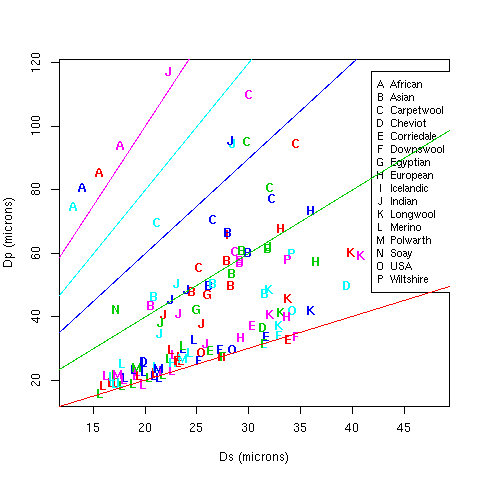
\includegraphics[width=1.0\textwidth]{dsdpalltype.png}
  \caption{Plot of breed means of secondary fibre diameter $D_{s}$ and primary fibre diameter $D_{p}$ for 126 flocks sampled by Carter(1968)~\cite{cart:68}. The breeds have been grouped into a {\em breed type} which in some cases is an individual breed and in other cases is a country of origin. The coloured lines represent various values of the ratio $D_{p}/D_{s}$. Red is $D_{p}/D_{s}=1$, green is $D_{p}/D_{s}=2$, blue is $D_{p}/D_{s}=3$, cyan is $D_{pi}/D_{s}=4$, and magenta is $D_{p}/D_{s}=5$.}
  \label{fig:dsdptype}
\end{figure}

%\end{document}


The use of the ratio $D_{p}/D_{s}$ was introduced by Dr Carter. We can see that it clearly separates the hairy African and Indian breeds, and that it also has high values for carpetwool breeds. Then there are a number of intermediate breeds with $D_{p}/D_{s}$ at about 2, including the Soay. The Soay sheep sampled by Dr Carter were of the Wooly Soay type. Finally there are the various strains of Merino, the Merino derived breeds, and the British Longwools and Downswools with $D_{p}/D_{s}$ between about 1.0 and 1.3. 

The ratio $D_{p}/D_{s}$ is not a complete descriptor of fleece diameter, it measures the tendency toward two-coatedness. There is also the average diameter of all the fibres $D_{p+s}$.  If we plot these two we get Figure~\ref{fig:DpovDsDps}.
%\documentclass{article}
%\usepackage{graphicx,subfigure}
%\begin{document}

\begin{figure}[!h]
  \centering
   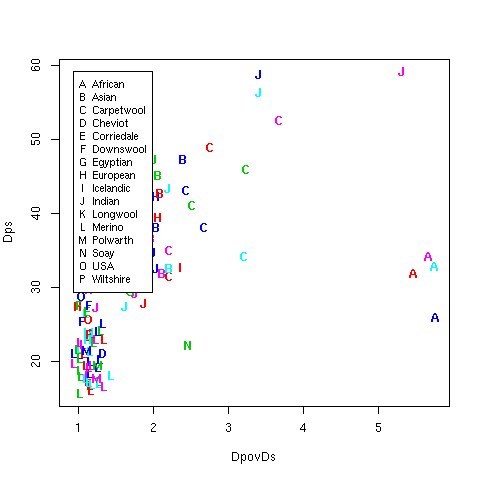
\includegraphics[width=1.0\textwidth]{DpovDsDps.png}
  \caption{Plot of breed means of  $D_{p}/D_{s}$ and mean fibre diameter $D_{ps}$ for 126 flocks sampled by Carter(1968)~\cite{cart:68}. The breeds have been grouped into a {\em breed type} which in some cases is an individual breed and in other cases is a country of origin. }
  \label{fig:DpovDsDps}
\end{figure}

%\end{document}


We see that the Merino lies in the lower left corner of Figure~\ref{fig:DpovDsDps} - neither two-coated nor coarse, relative to other breeds.

An alternative way of parameterizing two-coatedness and coarsness is to use rotation of axes in the graph og $D_{p}$ against $D_{s}$. If we rotate axes 45 degrees in Figure~\ref{fig:dsdptype} we get one axis running along the line $D_{p}/D_{s} = 1$, and the second axis at right angles to this. We call the first axis {\em L-axis} ( for large fibres), and the second axis {\em W-axis} (for wild two-coated type. A plot of W-axis aginst L-axis is given in Figure~\ref{fig:LWalltype}
%\documentclass{article}
%\usepackage{graphicx,subfigure}
%\begin{document}

\begin{figure}[!h]
  \centering
   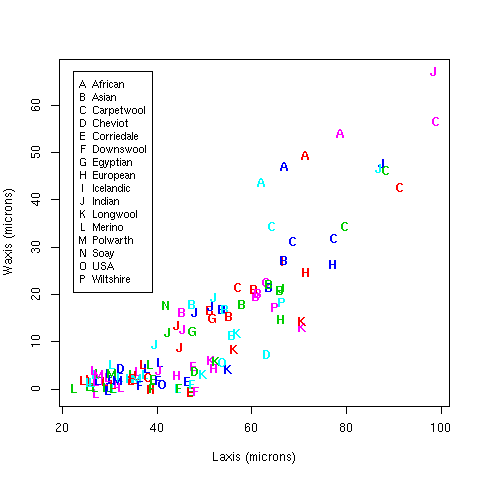
\includegraphics[width=1.0\textwidth]{LWalltype.png}
  \caption{Plot of breed means of secondary fibre diameter (Ds) and primary fibre diameter (Dp) for 126 flocks sampled by Carter(1968)~\cite{cart:68}. The axes have been rotated 45 degrees so that L-axis represents projections onto the line $D_{p}/D_{s} = 1$, and W-axis represents projections onto a line at right angles to the L-axis. The W-axis is interpreted a two-coatedness, and the L-axis is interpreted a large fibres. The breeds have been grouped into a {\em breed type} which in some cases is an individual breed and in other cases is a country of origin. }
  \label{fig:LWalltype}
\end{figure}

%\end{document}


We see the Merino still in the lower left corner, but the other breeds spaced in a manner indicating  a positive correlation of large fibres with a wild type two-coated fleece. The closest thing to a primitive domestic sheep in these data are the hair sheep from Africa and India, and they have W values of around 50-60 microns. The wooly Soay has a W value of only 20 microns, but its L value is only 40 microns, compared to 70-100 microns for the hair breeds. Merinos are distinguished from British Longwools and Downswools by a lower L value, Their W values are similar. On this criterion, Merinos are no further separated from two-coatedness than are modern British breeds - all 3 have similar W values ( and similar $D_{p}/D_{s}$.

Figure~\ref{fig:dsdptype} is not the full story. Dr Carter also introduced another ratio $N_{s}/N_{p}$  or the ratio of number of secondary follicles per unit area to number of primary follicles per unit area. If we look first at $N_{s}$ and $N_{p}$ (Figure~\ref{fig:NsNptype}) we see that the Merino ( and Merino derived breeds) is substantially different from all other breeds in $N_{s}$, and apart from a couple of Indian breeds with a high $N_{p}$, that is about the only significant difference. Most non-Merino breeds have $N_{p}$ between 1 and 3, and $N_{s}$ less than 20.
%\documentclass{article}
%\usepackage{graphicx,subfigure}
%\begin{document}

\begin{figure}[!h]
  \centering
   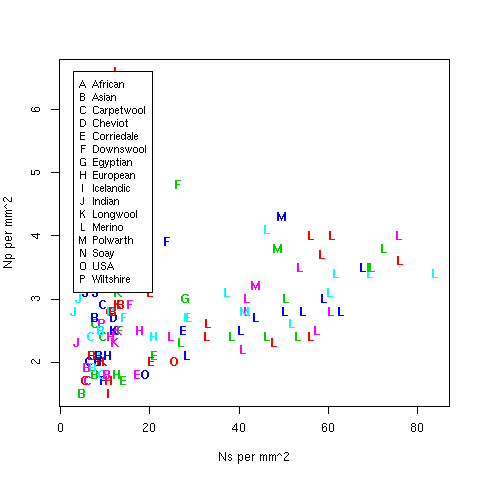
\includegraphics[width=1.0\textwidth]{NsNpalltype.png}
  \caption{Plot of breed means of secondary fibre density (Ns) and primary fibre density (Np) for 126 flocks sampled by Carter(1968)~\cite{cart:68}. The breeds have been grouped into a {\em breed type} which in some cases is an individual breed and in other cases is a country of origin. }
  \label{fig:NsNptype}
\end{figure}

%\end{document}


We mostly see data on $N_{s}$ presented as the ratio $N_{s}/N_{p}$ rather than as the straight density. This is supposed to avoid some of the errors involved in density measurement. It also reduces the presentation to one trait, because $N_{p}$ variation is small and probably reflects  variations in body growth. 

We can put the information from Carter's two ratios together, as in Figure~\ref{fig:NsovNpDpovDs}
%\documentclass{article}
%\usepackage{graphicx,subfigure}
%\begin{document}

\begin{figure}[!h]
  \centering
   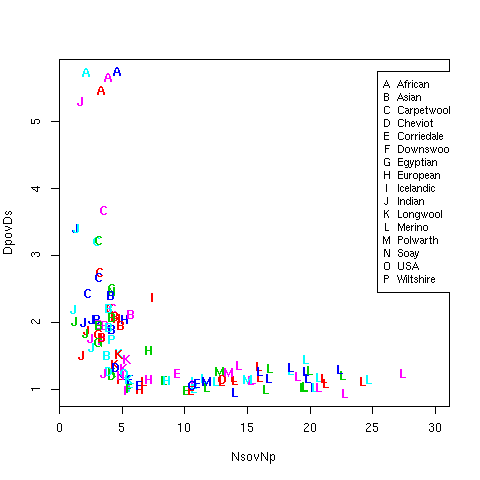
\includegraphics[width=1.0\textwidth]{NsovNpDpovDs.png}
  \caption{Plot of breed means of $N_{s}/N_{p}$ and $D_{p}/D_{s}$ for 126 flocks sampled by Carter(1968)~\cite{cart:68}. The breeds have been grouped into a {\em breed type} which in some cases is an individual breed and in other cases is a country of origin. }
  \label{fig:NsovNpDpovDs}
\end{figure}

%\end{document}


where we see the Merino distinguished mainly by a high $N_{s}/N_{p}$ ratio, but also by a low $D_{p}/D_{s}$ ratio. Figure~\ref{fig:NsovNpDpovDs} condenses everything that the Carter(1968)~\cite{cart:68} data have to say about breed differences in skin characteristics.

But Figure~\ref{fig:NsovNpDpovDs} is Carter's approach. For reasons that will become more apparent later, we prefer $D_{p}$ to $D_{p}/D_{s}$ ratio. So we repeat Figure~\ref{fig:NsovNpDpovDs} using $D_{p}$ instead of $D_{p}/D_{s}$ ratio in Figure~\ref{fig:NsovNpDp}
%\documentclass{article}
%\usepackage{graphicx,subfigure}
%\begin{document}

\begin{figure}[!h]
  \centering
   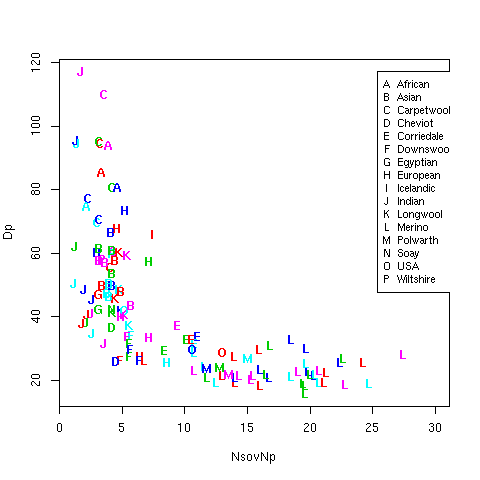
\includegraphics[width=1.0\textwidth]{NsovNpDp.png}
  \caption{Plot of breed means of $N_{s}/N_{p}$ and $D_{p}$ for 126 flocks sampled by Carter(1968)~\cite{cart:68}. The breeds have been grouped into a {\em breed type} which in some cases is an individual breed and in other cases is a country of origin. }
  \label{fig:NsovNpDp}
\end{figure}

%\end{document}


The relationship is still nonlinear, but less so, and the spread of points vertically is more uniform.

But this is not all that we know. We need to overlay these data with Ryder's summary of the stages in evolution of sheep breeds. We attermpt this in the next section

\section{Combining skin data with knowledge of breed evolution}
From Ryder's presentation of fibre data, and from various sources as indicated, we were able to put together some approximate measurements of sheep representing Ryder's stages of evolution of wool sheep. We have also added  SRS Merino data, because this modern development of the Australian Merino is becoming a significanltly different flece type. These are given in Table~\ref{tab:evolmeas}
%\documentclass{article}
%\usepackage{lscape}
%\begin{document}

\begin{table}[h]
\centering
\caption{Approximate measurements for sheep representing Ryder's 4 stages of Merino evolution, extended to the modern SRS Merino. Sources lines 1 to 3 Ryder(1992)~\cite{ryde:92}, line 4 Carter(1968)~\cite{cart:68}, line 5 Watts(2017)~\cite{watt:17}.}
\label{tab:evolmeas}
\vspace{0.1in}
\begin{tabular}{|p{0.6in}|p{0.6in}|p{0.4in}|p{0.4in}|p{0.6in}|p{0.7in}|p{0.7in}|}  \hline
  Stage &  Chronology &  Dp & Ds & S/P ratio & Medullation & Shedding  \\ \hline
  Wild   & Neolithic (10000-3000BC) & 80-200 & 14-16 & 3-5 & Outercoat kemp & Undercoat sheds \\ \hline
  Hairy Medium Wool & Bronze Age (3000 - 1000BC) & 40-140 & 18-28 & 4-5 & Outercoat hair & Undercoat sheds \\ \hline
  Generalised Medium Wool & Iron Age (1000BC - 700 AD) & 20-50 & 18-35 & 5-7  & No outercoat? & Secondaries continuous \\  \hline
  Finewool Merino & (1200AD - present) & 18-20 & 17-19 & 15-25 & No outercoat & Secondaries continuous\\  \hline
  SRS Fine Merino & (1990AD - present) & 14-17 & 17-19 & 25-40 & No outercoat & Secondaries continuous \\ \hline
\end{tabular}
\end{table}

%\end{document}

It is clear that there has been more than one significant change during evolution of the Merino. 
\begin{itemize}
\item reduction in diameter of primary fibres
\item loss of medullation in primary fibres in Bronze Age sheep
\item change from seasonal shedding to continuous growth of secondary fibres in Iron Age sheep
\item large increase in S/P ratio at the Finewool Merino step. Probably a mutation at this point.
\item further reduction of primary fibre diameter and further increase in S/P ratio at the SRS Merino step
\end{itemize}
There are some aspects of these changes which are not fully understood at the skin biology level. We do understand  how the reduced Dp in SRS Merino sheep leads to increased S/P Ratio - it is explained by the pre-papila cell theory of Moore et al (1998)~\cite{moor:98}. However the pre-papilla cell theory does not obviously explain the change from Wild to Hairy Medium Wool sheep - here we have a substantial reduction in Dp, but Ds increased and S/P was unaffected. Clearly changing Dp by removing the medulla does somethin different from reducing Dp in a non-medullated fibre. The relationship between Dp and number of papilla cells in the follicle may not be the same for medullated fibres.

Then we have another substantial reduction in Dp between Hairy Medium Wool and Generalised Medium Wool, and Ds actually increased further but S/P was probably unchanged. It would seem that to become continuous growing secondary fibres became coarser. 

Then there is the substantial jump in S/P Ratio at the Finewool Merino stage. This almost has to have been a single gene effect when it originally occurred. When Finewool Merino's are crossed with other breeds today we do not see single gene segregation with respect to S/P Ratio. This is because there has been many years of selection of modifying genes from 1200AD to present. The original mutant was probably the Rex gene. If you look at the effects of Rex gene on the coat of cats (Fraser(1953)~\cite{fras:53}) you see a substantial increase in S/P ratio and an increase in crimp in the fibres. Rex cats and rabbits have a {\em wavy} coat - Merino sheep have a more {\em wavy} coat than any other sheep breed. We might explain the increased S/P Ratio of Finewool Merinos by referring to the reduced Dp according to the pre-papilla cell theory, but this does not explain the change in crimp. In the SRS Merino the increased S/P Ratio is associated with a reduced crimp frequency, while in the Fine Merino the increased S/P Ratio is associated with an increase in crimp frequency. 

There is also a possibility thet the Finewool Merino may not have evolved from  the Generalised Medium Wool as Ryder proposed. There is no direct historical account of Merino origins. It suddenly appeared in Spain in about the 12th century and there is the possibility that it came from North Africa into Spain (Massy(2007)~\cite{mass:07}. There is therefore the possibility that it came directly from Hairy Medium Wool sheep, perhaps by a mutation, as suggested above. The Rex mutation in cats and rabbits turns a double coat into a fine single coat with crimped fibres, but it does not lead to continuous growing fibres. That would have to come from some other genetic change. Exactly what the lines of descent were does not matter here - we are looking at recurrence of ancestral characteristics not at how they were transmitted.

So we say that there are a number of issues to consider in Merino evolution. In spite of that we will attempt to reduce the comparisions to a couple of graphs in which we attempt to superimpose Ryder's long term picture on the available data. 

We start with the  plot of $D_{s}$ against $D_{p}$. Figure~\ref{fig:dsdptypea} is a repeat of Figure~\ref{fig:dsdptype} with the approximate measurements of $D_{s}$ and $D_{p}$ representing Ryder's 4 stages of Merino evolution from Table~\ref{tab:evolmeas} superimposed as coloured rectangles representing the approximate ranges of measurements. 
%\documentclass{article}
%\usepackage{graphicx,subfigure}
%\begin{document}

\begin{figure}[!h]
  \centering
   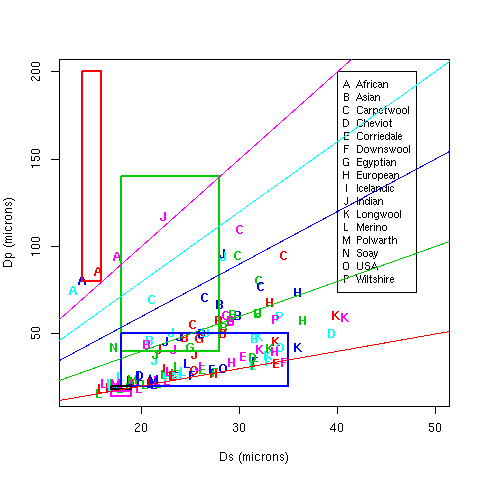
\includegraphics[width=1.0\textwidth]{dsdpalltypea.png}
  \caption{Plot of breed means of secondary fibre diameter $D_{s}$ and primary fibre diameter $D_{p}$ for 126 flocks sampled by Carter(1968)~\cite{cart:68}. The breeds have been grouped into a {\em breed type} which in some cases is an individual breed and in other cases is a country of origin. The coloured lines represent various values of the ratio $D_{p}/D_{s}$. Red is $D_{p}/D_{s}=1$, green is $D_{p}/D_{s}=2$, blue is $D_{p}/D_{s}=3$, cyan is $D_{p}/D_{s}=4$, and magenta is $D_{p}/D_{s}=5$. The coloured rectangles represent the approximate ranges of measurements for sheep representing Ryder\'s 4 stages of Merino evolution, plus the modern SRS Fine Merino. Red rectangle is Wild stage, green is Hairy Medium Wool, blue is Generalised Medium Wool, black is Finewool Merino, and magenta is SRS Fine Merino. }
  \label{fig:dsdptypea}
\end{figure}

%\end{document}


The first thing to note is that the superimposed rectangles seem to locate sensibly in relation to the Carter(1968)~\cite{cart:68} data. The African hair sheep are just at the lower tip of the Wild sheep rectangle. The green Hairy Medium Wool rectangle contains some carpet wool breeds and Asian ( ie Middle Eastern) and Indian breeds. The Soay, which was a Wooly Soay, is just to the left of the blue Generalised Medium Wool rectangle, which also embraces some of the British and European  breeds and the Merino derived breeds.

We now have an approximate criterion for judging whether a sheep is primitive. Figure~\ref{fig:dsdptypea} indicates that $D_{p}$ alone is the prime criterion. The entire evolutionary history of the Merino has been a story of decreasing $D_{p}$ at all stages, right down to the modern SRS Fine Merino with its $D_{p}$ less than $D_{s}$.  If we want to show that a particular Merino sample is showing signs of primitive characteristics, the first thing we should look at is  $D_{p}$ .

The story of how $D_{s}$ changes during Merino evolution is more complicated.  It increased between Wild sheep and Hairy Medium Wool sheep, increased slightly more in Generalised Medium Wool, then decreased again in Finewool Merino, and did not change going from there to SRS Fine Merino. We have to look at further data to understand this. There is a suggestion that the change to a continuous growth on secondary fibres from the undercoat led to an increase in secondary fibre diameter. There is also a suggestion that the large increase in $S/P$ ratio in Finewool Merino compared to previous stages led to finer secondary fibres. Again we have to look at further data. 

The use of $D_{p}/D_{s}$ is problematic. Over a broad range it is essentially the same as using $D_{p}$ - it clearly separates Wild from Hairy Medium Wool from Generalised Medium Wool, but it does not separate Generalised Medium Wool from Fine Merino or any of the other modern breeds.. 

If we move to the rotated version of the $D_{s}$ versus $D_{p}$ graph (Figure~\ref{fig:LWalltype}) and superimpose the data of Table~\ref{tab:evolmeas} we get Figure~\ref{fig:LWalltypea}.
%\documentclass{article}
%\usepackage{graphicx,subfigure}
%\begin{document}

\begin{figure}[!h]
  \centering
   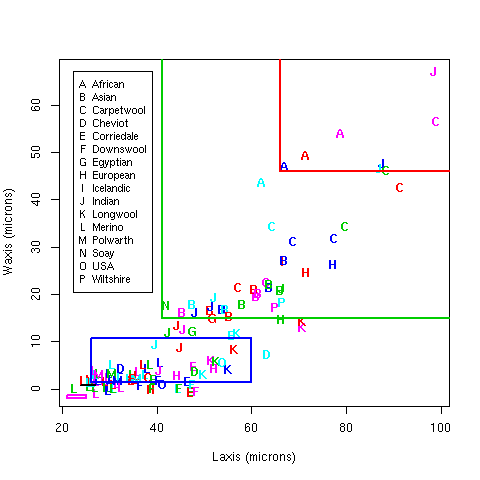
\includegraphics[width=1.0\textwidth]{LWalltypea.png}
  \caption{Plot of breed means of secondary fibre diameter (Ds) and primary fibre diameter (Dp) for 126 flocks sampled by Carter(1968)~\cite{cart:68}. The axes have been rotated 45 degrees so that L-axis represents projections onto the line $D_{p}/D_{s} = 1$, and W-axis represents projections onto a line at right angles to the L-axis. The W-axis is interpreted as two-coatedness, and the L-axis is interpreted as large fibres. The breeds have been grouped into a {\em breed type} which in some cases is an individual breed and in other cases is a country of origin. The coloured rectangles represent  the approximate ranges of L-axis and W-axis values for sheep representing Ryder\'s 4 stages of Merino evolution, plus the modern SRS Fine Merino. Red rectangle is Wild stage, green is Hairy Medium Wool, blue is Generalised Medium Wool, black is Finewool Merino, and magenta is SRS Fine Merino.}
  \label{fig:LWalltypea}
\end{figure}

%\end{document}


We see that the direction of evolution has been a reduction in both W-axis and L-axis. So neither of these alone is sufficient to describe observed evolutionary changes.

We need to look at $N_{s}/N_{p}$ ratio as well as $D_{p}$, so we redo Figure~\ref{fig:NsovNpDp} with the approximate measurements representing Ryder's 4 evolutionary stages from Table~\ref{tab:evolmeas} superimposed. This is shown in Figure~\ref{fig:NsovNpDpa}
%\documentclass{article}
%\usepackage{graphicx,subfigure}
%\begin{document}

\begin{figure}[!h]
  \centering
   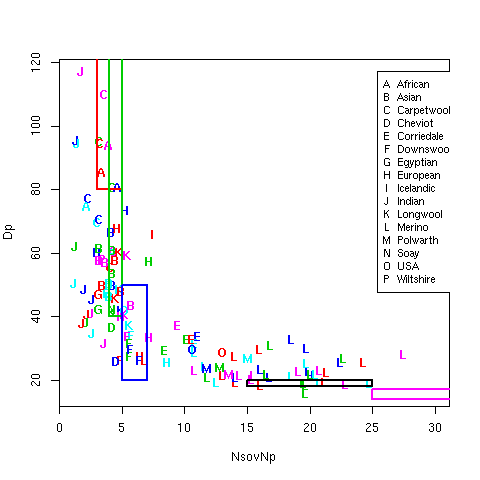
\includegraphics[width=1.0\textwidth]{NsovNpDpa.png}
  \caption{Plot of breed means of $N_{s}/N_{p}$ and $D_{p}$ for 126 flocks sampled by Carter(1968)~\cite{cart:68}. The breeds have been grouped into a {\em breed type} which in some cases is an individual breed and in other cases is a country of origin. The coloured rectangles represent the approximate ranges of measurements for sheep representing Ryder's 4 stages of Merino Evolution, plus the Modern SRS Fine Merino. Red rectangle is Wild stage, green is Hairy Medium Wool, blue is Generalised Medium Wool, black is Finewool Merino, and magenta is SRS Fine Merino.}
  \label{fig:NsovNpDpa}
\end{figure}

%\end{document}


It is now clear that evolution of the Fine Merino has involved reduction of $D_{p}$ and increase in $N_{s}/N_{p}$ at all stages. The dramatic increase in $N_{s}/N_{p}$ between Generalised Medium Wool and Fine Merino is the only {\em jump} in the evolutionary progression and suggests the possibility of a mutation, although there are breeds located in-between these two in Figure~\ref{fig:NsovNpDpa}. The other obvious point is that the SRS Merino is a continuation and extension of the same evolutionary process. 

If we refer back to Figure~\ref{fig:LWalltypea} we see that the L-axis and W-axis transform is just a linear version of Figure~\ref{fig:NsovNpDpa}. It uses $D_{s}$ instead of $N_{s}/N_{p}$, but they are nearly the same thing. Figure~\ref{fig:LWalltypea} also shows an evolutionary progression involving both L-axis and W-axis. Figure~\ref{fig:NsovNpDpa} is preferred, because of the conceptual difficulty of the L-axis and W-axis presentation.


\clearpage
\section{Discussion}
 We have reached a conclusion. If one wishes to decide whether a sheep or a flock shows primitive characteristics, one looks at three things
\begin{itemize}
\item diameter of primary fibres. The association of this with medullation and kemp formation can be noted.
\item $N_{s}/N_{p}$ ratio
\item lack of continuous growth of secondary fibres - ie shedding of secondaries.  Data on this are not often available.
\end{itemize}

There are sound biological reasons behind this choice. The pre-papilla cell theory of Moore et al (1998)~\cite{moor:98} shows that if follicles formed at primary sites use only a small number if pre-papilla cells in their development, then the remaining undifferentiated population of pre-papilla cells will be larger and will multiply to more cells by the time secondary follicles start to form. If there are more pre-papilla cells than are required by the secondary sites, then the remaining cells will form branching follicles, leading to a large $N_{s}/N_{p}$ ratio and fine secondary fibres.  This theory cleary fits with what has happened in going from Generalised Medium Wool to Fine Merino to SRS Merino. In the two earlier steps, which involve reduction of medullation of primary fibres, we can not be sure how $D_{p}$ would be related to the number of pre-papilla cells used by primary follicles. Between Wild sheep and Hairy Medium Wools, $D_{p}$ has reduced enormously, but $D_{s}$ has increased and $N_{s}/N_{p}$ has not changed much. It may be that reducing $D_{p}$ by reducing medullation is not accompanied by use of fewer pre-papilla cells. We simply have no data on this.

Why use two criteria ($D_{p}$ and $N_{s}/N_{p}$) that are highly related?  Well there is a temptation to look at the distribution of $D_{p}$ from fibre to fibre on one animal, and to note presence of some very coarse primary fibres which may not impact greatly on the mean diameter of primaries. What is the significance of a proportion of coarse primary fibres? Well it says that some primary follicles have followed a more ancient development path, while others have not. So there should be some impact on the mean $D_{p}$ and on $N_{s}/N_{p}$. Without going into distributions one can not quantify the impact. We should note that Ryder(1992)~\cite{ryde:92} emphasized the skewed shape of the diameter distribution of his Generalised Medium Wool sheep, and of the earlier stages. 

We have said nothing about why individual sheep or flocks might exhibit  ancestral or primitive characteristics. The genetics of atavism is another whole topic. The first step is to demonstrate that atavistic sheep actually occur and in which characteristics, and which flocks, is the phenomenon most obvious.  That is the task of the current rewrite of Jackson et al (1990)~\cite{jack:90}.

\clearpage
\begin{thebibliography}{99}

\bibitem{brow:68}
Brown, G.H., and Turner, Helen Newton. (1968) Response to selection in Australian Merino sheep. II. Estimates of phenotypic and genetic parameters for some production traits in Merino ewes and an analysis of the possible effects of selection on them. Aust. J. Agric. Res. 19:303-22

\bibitem{cart:43}
Carter, H.B. (1943) Studies in the biology of the skin and fleece of sheep. CSIRO (Aust) Bull. No. 164

\bibitem{cart:68}
Carter,H.B. (1968) Comparative Fleece Analysis Data for Domestic Sheep. The Principal Fleece Staple Values of Some Recognised Breeds. Agricultural Research Council, 1968
 
\bibitem{fras:53}
Fraser, A.S. (1953) A note on the growth of Rex and Angora coats. J. Genetics 521:237-42

\bibitem{fras:60}
Fraser A.S and Short B.F. (1960) The Biology of the Fleece. Animal Research Laboratories Technical Paper No 3. CSIRO Melbourne 1960.

\bibitem{jack:75}
Jackson, N., Nay, T, and Turner, Helen Newton (1975) Response to selection in Australian Merino sheep. VII Phenotypic and genetic parameters for some wool follicle characteristics and their correlation with wool and body traits. Aust. J. Agric. Res. 26:937-57

\bibitem{jack:15}
Jackson, N. (2015) Genetic relationship betweeen skin and wool traits in Merino sheep. Incomplete manuscript.

\bibitem{jack:16}
Jackson, N. and Watts, J.E. (2016) Staple crimp formation in the fleece of Merino sheep. Unpublished manuscript, 18 May 2016.

\bibitem{jack:90}
Jackson, N., Maddocks, I.G., Lax, J., Moore, G.P.M. and Watts, J.E. (1990) Merino Evolution, Skin Characteristics, and Fleece Quality. URL https://github.com/nevillejackson/atavistic-sheep/mev/evol.pdf 

\bibitem{mass:07}
Massy, C.(2007) The Australian Merino. Random House, Sydney, 2007
\bibitem{moor:89}
Moore G.P.M., Jackson, N., and Lax, J. (1989) Evidence of a unique developmental mechanism specifying bot wool follicle density and fibre size in sheep selected for single skin and fleece characters. Genet. Res. Camb. 53:57-62

\bibitem{moor:98}
Moore, G.P.M., Jackson, N., Isaacs, K., and Brown, G (1998) J. Theoretical Biology 191:87-94


\bibitem{nayj:73}
Nay, T. and Jackson, N. (1973) Effect of changes in nutritional level on the depth and curvature of wool follicles in Australian Merino sheep. Aust. J. Agric. Res. 24:439-447

\bibitem{onio:62}
Onions, W.J. (1962) Wool: an introduction to its properties, varieties, uses
     and production. Ernest Benn limited, London, 1962

\bibitem{rprog:13}
R Core Team (2013). R: A language and environment for statistical
  computing. R Foundation for Statistical Computing, Vienna, Austria.
  ISBN 3-900051-07-0, URL http://www.R-project.org/.

\bibitem{ryde:81}
Ryder, M.L. (1981) A Survey of European Primitive Breeds of Sheep. Ann. Genet. Sel. anim. 13(4):381-418

\bibitem{ryde:92}
Ryder, M.L. (1992) The interaction between biological and technological change during the development of different fleece types in sheep. Anthropozoologica 16:131-140

\bibitem{turn:53}
Turner, Helen Newton, Hayman, R.H., Riches, J.H., Roberts, N.F., and Wilson, L.T. (1953) Physical definition of sheep and their fleece for breeding and husbandry studies: with particular reference to Merino sheep. CSIRO Div. Anim. Hlth. Prod. Div. Rept. No. 4 (Ser SW-2 mimeo)


\bibitem{turn:70}
Turner, Helen Newton, Brooker M.G. and Dolling, C.H.S (1970) Response to selection in Australian Merino sheep. III Single character selection for high and low values of wool weight and its components. Aust.J.Agric.Res. 21:955-84

\bibitem{vonb:48}
Von Bergen, W. and Mauersberger, H.R.(1948) American Wool Handbook. 2nd ed. Barnes, New York.

\bibitem{watt:17}
Watts, J.E. (2017) Personal communication.
\end{thebibliography}
\end{document}
